






%\chapter*{Part I Conclusion}{Introduction de la Partie I}
\chapter*{Conclusion de la Partie I : une définition de la co-évolution}


% to have header for non-numbered introduction
% \markboth{Conclusion of Part I}{Conclusion of Part I}
\markboth{Conclusion de la Partie I}{Conclusion de la Partie I}


%\headercit{}{}{}


%La première conclusion marquante de cette première partie se résume parfaitement dans le meme suivant :


%{\centering
%\medskip
%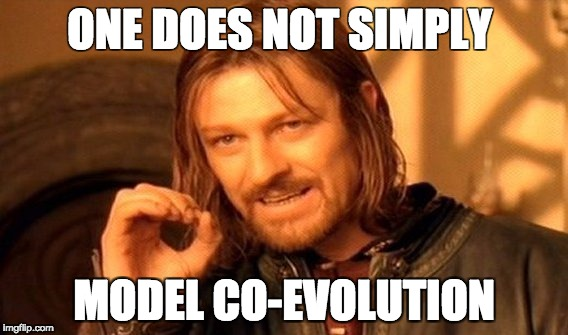
\includegraphics[width=\textwidth]{Figures/Art/onedoesnotsimply.jpg}
%\medskip
%}

Cette première partie nous permet de cerner bien plus précisément notre question de recherche. En effet, le premier chapitre nous a permis de dresser un portrait de la diversité des processus impliqués et des échelles temporelles et spatiales concernées. Le deuxième chapitre nous a donné une vue très générale des modélisations existantes et de leur contexte scientifique précis. Enfin, le troisième chapitre positionne la question de manière épistémologique, apporte un éclairage multi-disciplinaire sur la co-évolution, et clarifie la complexité dans laquelle nous nous situons. Cela nous permet d'ouvrir sur les directions à prendre par la suite pour mener à bien l'entreprise de modélisation de la co-évolution.


\subsection*{Defining co-evolution}{Définir la co-évolution}

Après l'aperçu de la littérature donné en~\ref{sec:modelingsa}, incluant différents degrés de couplage entre les composantes des réseaux et territoires, nous sommes tout d'abord en mesure de préciser ce que nous entendrons par \emph{modéliser la co-évolution}, en fixant une définition de la co-évolution au regard de l'aperçu multi-disciplinaire mené en~\ref{sec:epistemology}.

Nous proposons l'entrée suivante pour le cas spécifiques des réseaux de transport et des territoires, qui fait écho au trois points essentiels (existence de processus évolutif, définition des entités ou des populations, isolation de sous-systèmes dans le temps et l'espace) que nous avons dégagé en~\ref{sec:epistemology}. Celle-ci vérifie les trois spécifications suivantes.

Dans un premier temps, les processus évolutifs correspondent aux transformations des composantes du système territorial aux différentes échelles : transformation sur le temps long des villes, de leur réseaux, transmission entre villes des caractéristiques socio-économiques portées par les agents microscopiques mais aussi transmission culturelle, reproduction et transformation des agents eux-mêmes (firmes, ménages, opérateurs)\footnote{Cette liste s'appuie sur les hypothèses de la théorie évolutive que nous avons déjà introduite brièvement et que nous développerons à part entière en Chapitre~\ref{ch:evolutiveurban}. Elle ne peut être exhaustive, puisque ce qui ferait ``l'ADN d'une ville'' reste une question ouverte comme nous le rappelle \noun{Denise Pumain} dans un entretien dédié~\ref{app:sec:interviews}.}.

Ces processus évolutifs peuvent impliquer une co-évolution. Au sein d'un système territorial, pourront être en co-évolution à la fois : (i) des entités données (telle infrastructure et telles caractéristiques de tel territoire par exemple, c'est-à-dire des individus), lorsque leur influence mutuelle sera circulairement causale (à l'échelle leur correspondant) ; (ii) des populations d'entités, ce qui se traduira par exemple par tel type d'infrastructure et telle composante territoriale co-évoluent au niveau statistique dans une région géographique donnée ; (iii) l'ensemble des composantes d'un système à petite échelle géographique lorsqu'il existe de fortes interdépendances globales. Notre vision est donc fondamentalement \emph{multi-échelles} et articule différentes significations à différentes échelles.


Enfin, la contrainte d'une isolation implique, en lien avec le point précédent, que la co-évolution et l'articulation des significations auront un sens s'il existe des isolations spatio-temporelle de sous-systèmes où s'effectuent les différentes co-évolutions, ce qui est en accord direct avec un vision en \emph{Systèmes de systèmes multi-échelles}.

% dernier point : lien avec la notion de morphogenese : a appuyer dans intro de II

Cette définition élargie constituera notre référence par la suite lorsqu'on parlera de co-évolution des réseaux de transport et des territoires.

%L'une de nos contributions en synthèse faite en~\ref{sec:theory} sera de formaliser cette définition au regard des résultats que nous aurons obtenus. Elle constituera jusque là notre base d'investigation.


Nous pouvons alors synthétiser les résultats fondamentaux de cette première partie dans les deux faits marquants suivants :
\begin{enumerate}
	\item L'hypothèse de la co-évolution des réseaux de transport et des territoires est supportée d'un point de vue théorique et thématique, et nous en construisons une définition précise.
	\item La co-évolution reste très peu explorée dans la littérature de modélisation urbaine, les caractéristiques des disciplines concernées et leurs interactions pouvant en être une cause.
\end{enumerate}

Développons à présent les perspectives qui s'ouvrent à ce stade.


\subsection*{On the need of an empirical characterization}{Du besoin d'une caractérisation empirique}

La signification la plus large, c'est à dire l'interdépendance généralisée, trouve vite ses limites si les motifs ne sont pas finement caractérisés. Elle permet comme prémisse épistémologique de considérer certaines ontologies et certaines démarches de modélisation, mais permet difficilement de comprendre finement la structure et les processus d'un système. Il s'agira alors de descendre en généralité et de considérer des sous-systèmes, au sein desquels on peut s'intéresser à la co-évolution d'entités et de population. Une compréhension à ce niveau nécessite une caractérisation empirique fine, sans quoi notre distinction n'aurait pas de sens. Une question qui s'ouvre, et que nous devrons traiter par la suite, est alors quelles sont les méthodes empiriques possibles pour caractériser une co-évolution entre entités ou populations d'entités.


\subsection*{Two complementary directions}{Deux pistes complémentaires}


% combiner : empirique (carac empirique) et modeling / deux echelles (plusieurs, mais au min deux) / deux stream d'inclusion dans les modeles : idem ? / coevol amene deja l'idee d'isolation et de sous systeme indep : morphogenesis
%  -> unexplored streams from the literature - details why particularly suited in intro Part II . objectif de l'inclusion dans les modèles


L'état de l'art fait en~\ref{sec:modelingsa} ci-dessus témoigne d'une faiblesse de la littérature dans le domaine du couplage fort entre évolution des territoires et croissance des réseaux, vu la portée restreinte et la disparité des travaux revus. Les lacunes à combler sur ce point seraient donc liées à l'introduction de modèles fortement couplés dans le temps plus ou moins multi-processus et multi-échelles, pour lesquels une partie des modèles décrits en~\ref{sec:modelingsa} puis en~\ref{sec:modelography} sont précurseurs.


Les premières recherches exploratoires que nous allons mener doivent répondre à différentes tensions conceptuelles qui découlent des conclusions que nous venons de tirer :
\begin{itemize}
	\item permettre à la fois une approche empirique, et en particulier un méthode de caractérisation, ainsi qu'une approche de modélisation ;
	\item permettre la prise en compte de différentes échelles ;
	\item permettre l'inclusion d'ontologies pour les territoires et pour les réseaux qui ne sont pas toujours directement compatibles.
\end{itemize}

Les échelles seront notamment une échelle mesoscopique et une échelle macroscopique puisque comme nous l'avons suggéré en~\ref{sec:reproducibility} avec l'étude des flux de trafic, et comme le montre \cite{yasmin2017macro} pour la validation d'un modèle d'activités, l'échelle microscopique présente des trajectoires complexes difficiles à reproduire.


Nous choisirons pour répondre simultanément à ces différentes problématiques une stratégie originale de double entrée thématique.



% why does not study mobility et suggestion preliminaire de meso-macro scales only. -> conclusion Partie I
%\bpar{}
%{
%Il faut aussi garder à l'esprit que le transport en lui-même est différent des réseaux de transport\comment[FL]{en quoi estce un argument ?}, puisqu'il correspond à l'utilisation de ceux-ci par les agents territoriaux. Dans une grande partie des approches que nous décrirons par la suite, et typiquement les approches appliquée en planification urbaine, la modélisation du transport s'axe sur des question de demande, d'offre, de congestion, c'est à dire à des échelles relatives à la mobilité, et est liée au réseau mais ne se concentre pas directement sur celui-ci\comment[FL]{ce n'est pas clair $\rightarrow$ la croissane du reseau ?, l'usage du reseau ? la croissance de l'usage du reseau ?} comme notre positionnement propose\comment[AB]{$\simeq$}.
%}


